\documentclass[12pt,a4paper,oneside]{report}
% ============================================================
% PREAMBLE -- Internship report PFA1 (UM6P format), English version
% Police Carlito (clone metrique libre de Calibri), taille 12.
% Compiler avec XeLaTeX / tectonic.
% ============================================================

\usepackage[english]{babel}
\usepackage[margin=2.4cm, top=2.6cm, bottom=2.4cm]{geometry}

% ------------------------------------------------------------
% POLICE : Carlito = clone metrique libre de Calibri
% ------------------------------------------------------------
\usepackage{fontspec}
\setmainfont{Carlito}[
  Extension      = .ttf,
  Path           = /usr/share/fonts/carlito/,
  UprightFont    = Carlito-Regular,
  BoldFont       = Carlito-Bold,
  ItalicFont     = Carlito-Italic,
  BoldItalicFont = Carlito-BoldItalic
]
\setmonofont{DejaVu Sans Mono}[Scale=0.85]

\usepackage{amsmath}
\usepackage{amssymb}

\usepackage{graphicx}
\graphicspath{{../plots/}{./figures/}}

\usepackage{booktabs}
\usepackage{array}
\usepackage{tabularx}
\usepackage{adjustbox}
\usepackage{enumitem}
\usepackage[table]{xcolor}
\usepackage{caption}
\usepackage{float}

\usepackage{tikz}
\usetikzlibrary{arrows.meta, positioning}

\usepackage{fancyhdr}
\usepackage{titlesec}
\usepackage{titletoc}

\usepackage[hidelinks]{hyperref}

% Headings required by the school's guidelines
\addto\captionsenglish{%
  \renewcommand{\listfigurename}{List of Figures}%
  \renewcommand{\listtablename}{List of Tables}%
  \renewcommand{\bibname}{References}%
}

% ------------------------------------------------------------
% PALETTE
% ------------------------------------------------------------
\definecolor{accent}{RGB}{17,112,120}      % teal -- titres
\definecolor{caplabel}{RGB}{26,105,150}    % bleu -- etiquettes figures/tables
\definecolor{umorange}{RGB}{215,74,42}     % orange UM6P -- filets
\definecolor{rulegray}{RGB}{120,120,120}

% ------------------------------------------------------------
% LEGENDES : etiquette coloree en gras, texte justifie
% ------------------------------------------------------------
\captionsetup{
  font=small,
  labelfont={bf,color=caplabel},
  labelsep=period,
  justification=justified,
  singlelinecheck=false,
  skip=6pt
}
\captionsetup[figure]{justification=justified}
\captionsetup[table]{justification=justified}

\renewcommand{\arraystretch}{1.15}
\newcolumntype{Y}{>{\centering\arraybackslash}X}
\newcommand{\rowrule}{\midrule[0.2pt]}

% ------------------------------------------------------------
% EN-TETES / PIEDS
% ------------------------------------------------------------
% Chaque style est defini par \fancypagestyle et re-execute son propre corps
% a l'activation : sans cela, le \fancyhf{} du style "plain" efface
% definitivement les en-tetes du style principal (registres globaux fancyhdr).
\setlength{\headheight}{15pt}

\fancypagestyle{main}{%
  \fancyhf{}%
  \renewcommand{\headrulewidth}{0.4pt}%
  \renewcommand{\footrulewidth}{0pt}%
  \fancyhead[L]{\small\nouppercase{\leftmark}}%
  \fancyhead[R]{\small Internship Report -- PFA1}%
  \fancyfoot[C]{\thepage}%
}

\fancypagestyle{plain}{%
  \fancyhf{}%
  \renewcommand{\headrulewidth}{0pt}%
  \renewcommand{\footrulewidth}{0pt}%
  \fancyfoot[C]{\thepage}%
}

\pagestyle{main}

% ------------------------------------------------------------
% TITRES
% ------------------------------------------------------------
\titleformat{\chapter}[display]
  {\normalfont\huge\bfseries\color{accent}}
  {\large\chaptertitlename\ \thechapter}
  {8pt}
  {\Huge}
  [{\color{umorange}\titlerule[1.2pt]}]
\titlespacing*{\chapter}{0pt}{-28pt}{16pt}

\titleformat{\section}
  {\large\bfseries\color{accent}}
  {\thesection}{0.7em}{}
\titlespacing*{\section}{0pt}{2.8ex plus 1ex minus .2ex}{1.2ex plus .2ex}

\titleformat{\subsection}
  {\normalsize\bfseries\color{accent}}
  {\thesubsection}{0.7em}{}
\titlespacing*{\subsection}{0pt}{2.2ex plus 1ex minus .2ex}{0.9ex plus .2ex}

\titleformat{\subsubsection}
  {\normalsize\bfseries}
  {\thesubsubsection}{0.7em}{}
\titlespacing*{\subsubsection}{0pt}{1.8ex plus 1ex minus .2ex}{0.7ex plus .2ex}

% ------------------------------------------------------------
% STYLE TIKZ partage par les schemas
% ------------------------------------------------------------
\tikzset{
  rbox/.style={draw, rounded corners, fill=accent!10, align=center,
               minimum height=1.0cm, text width=#1, font=\small},
  rbox/.default=2.6cm,
  flow/.style={-{Latex[length=2.2mm]}, thick}
}

% ------------------------------------------------------------
% DIVERS
% ------------------------------------------------------------
\setlength{\parskip}{0.42em}
\setlength{\parindent}{0pt}
\setlist{itemsep=2pt, topsep=3pt, parsep=0pt}


\begin{document}

% ============================================================
% COVER PAGE
% ============================================================
\begin{titlepage}
\thispagestyle{empty}
\centering


\includegraphics[width=0.50\textwidth]{um6p_college_of_computing_logo.png}

\vspace{1.0cm}

{\large Mohammed VI Polytechnic University}\\[2pt]
{\large College of Computing -- Benguerir}\\[2pt]
{\large Programme: Artificial Intelligence \& Data Science}

\vspace{1.2cm}

{\Large\bfseries INTERNSHIP REPORT}\\[4pt]
{\large End-of-Year Project, Year 1 (PFA1)}

\vspace{1.0cm}
{\color{rulegray}\rule{0.86\textwidth}{0.8pt}}
\vspace{0.8cm}

{\LARGE\bfseries\color{accent}
Machine-Learning-Augmented Shock-Capturing\\[6pt]
Schemes: from Imitation Learning\\[6pt]
to an Unrolled Physics Loss\\}

\vspace{0.8cm}
{\color{rulegray}\rule{0.86\textwidth}{0.8pt}}

\vspace{1.2cm}

{\large Carried out at}\\[4pt]
{\large\bfseries UM6P -- COLLEGE OF COMPUTING}\\[4pt]
{\large From 1 June to 1 August 2026}

\vspace{1.4cm}

\noindent
\begin{minipage}[t]{0.48\textwidth}
\raggedright
{\bfseries Written by:}\\[3pt]
Yasser BAOUZIL
\end{minipage}
\hfill
\begin{minipage}[t]{0.48\textwidth}
\raggedleft
{\bfseries Host supervisor:}\\[3pt]
Mr Radouan BOUKHARFANE\\[8pt]
{\bfseries Academic supervisor:}\\[3pt]
Mr Radouan BOUKHARFANE
\end{minipage}

\vfill
{\large Academic year 2025 -- 2026}

\end{titlepage}

% ============================================================
% FRONT MATTER
% ============================================================
\pagenumbering{roman}
\setcounter{page}{1}
\pagestyle{plain}

\chapter*{Acknowledgements}
\addcontentsline{toc}{chapter}{Acknowledgements}
\markboth{Acknowledgements}{}

I would like to express my sincere gratitude to everyone who made this
internship possible and rewarding.

My thanks go in particular to Mr Radouan Boukharfane, who supervised this
internship both professionally and academically, for entrusting me with a
genuine research question rather than a fixed specification, for proposing the
central idea behind the second phase of the project -- the unrolled physics
loss -- and for the precision of his feedback, notably on the correct
definition of the BVD term, which unlocked a key stage of the work.

I also thank the teaching staff and the administration of the College of
Computing at Mohammed~VI Polytechnic University for the training I received and
for the working environment made available to me over these two months.

\chapter*{Abstract}
\addcontentsline{toc}{chapter}{Abstract}
\markboth{Abstract}{}

This report presents the work carried out during my end-of-year internship
(PFA1) at the College of Computing of Mohammed~VI Polytechnic University. The
assignment concerned machine-learning-augmented shock-capturing numerical
schemes: determining whether a neural network can improve the reconstruction
step of a classical WENO/TENO-type scheme for hyperbolic conservation laws.

The work is organised into four strands. The first reproduces the published
results of the WENO5-NN scheme of Stevens \& Colonius in order to establish a
verified baseline. The second extends the same approach to TENO5 through
imitation training, and reveals a structural ceiling: a network trained to copy
a teacher scheme's decision cannot, by construction, surpass it. This finding
motivated the second phase of the internship, based on an \emph{unrolled
physics loss} proposed by the supervisor: instead of a one-shot imitation
label, the network is unrolled over $K$ real simulation steps and evaluated
directly against the true solution. This formulation required a complete,
differentiable rewrite of the project's numerical core in JAX. The third and
fourth strands apply this loss to the scalar benchmarks (advection, Burgers)
and then to the Euler system (Sod, Shu--Osher).

The main result is a clear win on the canonical scalar benchmarks ($3.5\%$ gain
on advection, $18.6\%$ on Burgers, outside the training distribution) and a
first outright win on the Euler system ($1.84\%$ on Shu--Osher), obtained
through a convex mixing mechanism driven by a dedicated head. The second
result, negative but equally instructive, is that the Sod case remains a
near-tie unfavourable to the network, and that a direct sweep of the mixing
coefficient shows this to be a structural limit of the learned scheme rather
than a calibration gap.

\vspace{0.6em}
\textbf{Keywords:} WENO/TENO schemes, hyperbolic conservation laws, shock
capturing, deep learning, automatic differentiation, JAX, unrolled physics
loss, Euler system.

\tableofcontents
\listoffigures
\addcontentsline{toc}{chapter}{List of Figures}
\listoftables
\addcontentsline{toc}{chapter}{List of Tables}

% ============================================================
% BODY
% ============================================================
\cleardoublepage
\pagenumbering{arabic}
\setcounter{page}{1}
\pagestyle{main}

\chapter*{Introduction}
\addcontentsline{toc}{chapter}{Introduction}
\markboth{Introduction}{}

As part of the first year of the engineering cycle at the College of Computing
of Mohammed~VI Polytechnic University, I completed a two-month end-of-year
internship, from 1~June to 1~August~2026, within the institution itself, under
the supervision of Mr Radouan Boukharfane.

The numerical simulation of compressible flows faces a long-standing and
structuring difficulty: in the presence of a shock, a discontinuous solution
appears in finite time even from perfectly smooth initial data. A high-order
numerical scheme applied naively then produces spurious oscillations (the Gibbs
phenomenon) which can render the solution non-physical -- negative density or
pressure -- and cause the computation to diverge. Schemes of the ENO/WENO/TENO
family solve this problem by adapting the reconstruction locally: they detect
the sub-stencils crossed by a discontinuity and reduce, or cancel entirely,
their contribution.

This detection relies on analytical smoothness indicators and on empirically
fixed constants. It is precisely this point that machine learning promises to
improve: if the keep/discard decision of a classical scheme is a nonlinear
function of the local solution values, a neural network can in principle
approximate it, or even do better. Several published works have explored this
avenue, with encouraging but mixed results.

The question put to this internship was therefore the following: \emph{can a
neural network genuinely outperform a classical shock-capturing scheme,
measured against the true solution and on canonical benchmarks?} This report
answers that question through four experimental strands, and documents the
failures as thoroughly as the successes -- the former having decisively shaped
the direction of the work.

The report is organised as follows. Chapter~\ref{chap:company} presents the
host institution. Chapter~\ref{chap:context} sets out the scientific
background, the project scope and the methodology adopted.
Chapter~\ref{chap:design} describes the design of the solution, from the
network architecture to the differentiable JAX rewrite.
Chapter~\ref{chap:work} details the four experimental strands.
Chapter~\ref{chap:results} consolidates the results and offers a critical
analysis.

% ============================================================
\chapter{Presentation of the Host Institution}
\label{chap:company}

\section{Field of activity}

Mohammed~VI Polytechnic University (UM6P) is a Moroccan higher education and
research institution, based mainly on the Benguerir campus in the
Marrakech-Safi region. Oriented towards applied research and innovation, it
covers a broad spectrum of fields ranging from materials science and
agriculture to digital sciences.

The internship took place within the \textbf{College of Computing}, one of the
university's components, dedicated to information science and technology:
computer science, artificial intelligence, data science and scientific
computing. Unlike a company, the primary purpose of this structure is not the
production of a commercial service but the production of knowledge: scientific
publications, doctoral supervision, and the development of tools and methods
reusable by the scientific community.

The project carried out during this internship falls within the area of
\emph{scientific computing and computational fluid dynamics} (CFD), at the
intersection of classical numerical analysis and machine learning -- a rapidly
expanding field in which learning methods are used not to replace numerical
solvers, but to improve targeted components of them.

\section{Organisational structure}

UM6P is organised into thematic \emph{colleges} and institutes, each grouping
teaching programmes and research teams around one field. The College of
Computing follows this logic: it combines a teaching mission (engineering
programmes, including the Artificial Intelligence \& Data Science track I am
enrolled in) and a research mission organised into teams attached to
faculty researchers.

The supervision of an intern there follows a direct pattern, with no
intermediate hierarchy: the student is attached to a faculty researcher who
defines the topic, steers the work and evaluates its results. In my case,
Mr Radouan Boukharfane acted simultaneously as host supervisor and academic
supervisor. This arrangement had one important practical consequence for how
the internship unfolded: it was steered by scientific objectives and by the
validation of measured results, rather than by delivery milestones.

\section{Professions represented}

The professions represented in the immediate environment of the internship
belong mainly to research and scientific computing:

\begin{itemize}
  \item \textbf{Faculty researcher} -- defines research directions, supervises
  and publishes. This is my supervisor's profession.
  \item \textbf{Doctoral / postdoctoral researcher} -- conducts a research
  programme over several years.
  \item \textbf{Research / scientific computing engineer} -- implements and
  optimises simulation codes, ensures the reproducibility of experiments.
  \item \textbf{Data scientist / machine learning engineer} -- designs, trains
  and evaluates models; the profile my own training is directed towards, and
  the one matching the hybrid nature of the subject treated here.
\end{itemize}

The work carried out during this internship sits precisely at the intersection
of the last two professions: it demanded command of a numerical solver
(reconstruction schemes, time integration, stability) as much as of a machine
learning pipeline (architecture design, loss function, training, evaluation).

% ============================================================
\chapter{Scientific Background and Project Scope}
\label{chap:context}

\section{Scientific background: finite volumes and conservation laws}
\label{sec:background-fv}

A scalar hyperbolic conservation law is written
\[
\partial_t u + \partial_x f(u) = 0,
\]
and the compressible Euler system is its vector generalisation, where $u$
gathers the conserved variables (density, momentum, energy) and $f(u)$ is the
associated physical flux. Both are solved here by the method of lines: the
domain is divided into $N$ cells, each cell $i$ stores an average $u_i$, and
the equation is advanced by estimating the flux at every interface $i+1/2$ and
then integrating
\[
\frac{d u_i}{dt} = -\frac{1}{\Delta x}\left(\hat f_{i+1/2} - \hat f_{i-1/2}\right)
\]
in time, using a third-order Runge--Kutta integrator (SSPRK3). This integrator
has the property of being a convex combination of explicit Euler steps, which
guarantees that it does not amplify an already non-oscillatory state. The flux
is furthermore split into an upwind and a downwind part (Lax--Friedrichs
splitting) before reconstruction, so that upwinding remains well defined even
where the wave speed changes sign.

The whole numerical difficulty lies in $\hat f_{i+1/2}$: reconstructing a
high-order estimate at the interface without introducing oscillations near a
discontinuity. For the Euler system, the reconstruction is applied not to the
conserved variables directly, but to the \emph{characteristic fields} of the
system, obtained through a local change of basis that decouples the three
waves. This detail has an important consequence later on: that change of basis
depends on the solution itself, so an imperfect reconstruction degrades the
basis used at the next step (Section~\ref{sec:instability}).

\section{ENO, WENO and TENO reconstructions}
\label{sec:background-schemes}

The three schemes all reconstruct $\hat f_{i+1/2}$ from the same 5-point
stencil $f_{i-2},\dots,f_{i+2}$, split into three overlapping 3-point candidate
sub-stencils. Each candidate provides, by polynomial interpolation, its own
estimate of the value at the interface. What distinguishes the three schemes is
solely the \emph{way} these three estimates are combined.

\textbf{ENO} \cite{harten1987} retains only the smoothest candidate and
discards the other two. Since this choice is discontinuous with respect to the
data, it limits the order of accuracy attainable in smooth regions.

\textbf{WENO} \cite{jiang1996} replaces this hard choice with a convex
combination of all three candidates:
\[
\hat f_{i+1/2} = \sum_{k=0}^{2} w_k\, \hat f_{k,i+1/2}, \qquad
w_k = \frac{\alpha_k}{\sum_{l}\alpha_l}, \qquad
\alpha_k = \frac{d_k}{(\beta_k + \varepsilon)^{q}} .
\]
The $d_k$ are fixed weights, called \emph{optimal}, which recover the full
fifth-order reconstruction when the three candidates agree; $\varepsilon$
prevents division by zero. Each $\beta_k$ is a \textbf{smoothness indicator}: a
sum of squared finite differences measuring how ``agitated'' candidate $k$ is.
The mechanism fits in one sentence: near a discontinuity, the candidate crossed
by it has a large $\beta_k$, hence a weight $w_k$ that collapses towards zero;
in a smooth region, all $\beta_k$ are small and comparable, $w_k \to d_k$, and
fifth-order accuracy is recovered.

\textbf{TENO} \cite{fu2016} keeps this mechanism but replaces the gradual
weighting with a \emph{binary} decision. The $\beta_k$ are first normalised
into a measure $\chi_k \in [0,1]$, then compared against a fixed threshold
$C_T$:
\[
\delta_k = \begin{cases} 0, & \text{if } \chi_k < C_T \quad (\text{candidate discarded}) \\[2pt]
                         1, & \text{otherwise} \quad (\text{candidate kept}), \end{cases}
\qquad
w_k = \frac{d_k\,\delta_k}{\sum_{l}d_l\,\delta_l} .
\]
A candidate below the threshold is therefore discarded \emph{entirely} rather
than merely down-weighted. This is what gives TENO5 sharper discontinuity
capturing than WENO5 at comparable computational cost, and it is why this is
the scheme the internship seeks to improve.

\textbf{It is the decision $\delta_k$ that this internship trains a neural
network to replace}: given the normalised 5-point stencil, output for each of
the three candidates the probability that it should be discarded.

\section{From the real flow to a one-dimensional signal}

A shock is not a mathematical abstraction: it is an observable physical
discontinuity. Panel~(a) of Figure~\ref{fig:pipeline} gives a direct image of
one -- a schlieren photograph of a T-38 in supersonic flight at Mach~1.1, taken
by NASA \cite{nasa1993}. The schlieren technique makes density gradients in the
air visible: the dark oblique bands are the shock waves attached to the
aircraft.

By taking a \textbf{one-dimensional cut} through this flow (red line), one
obtains the signal $u(x)$ of panel~(b): long smooth regions separated by a few
very steep transitions. This is exactly the structure that ENO/WENO/TENO
schemes are designed to handle, and it is also what makes the problem hard: a
high-order scheme is excellent on the smooth regions and catastrophic near the
transitions, where it produces spurious oscillations.

All the work of this internship therefore bears on a single question, posed on
this 1D signal: \emph{how does one reconstruct the value at the interface
between two cells, with high order where the signal is smooth, without
oscillating where it is not?}

\medskip
Figure~\ref{fig:pipeline} unrolls the complete chain on this real case, from
the physical flow to the advance in time. The first two steps constitute a
set-up performed once; the following ones form the loop repeated at every time
step.

\begin{figure}[H]
\centering
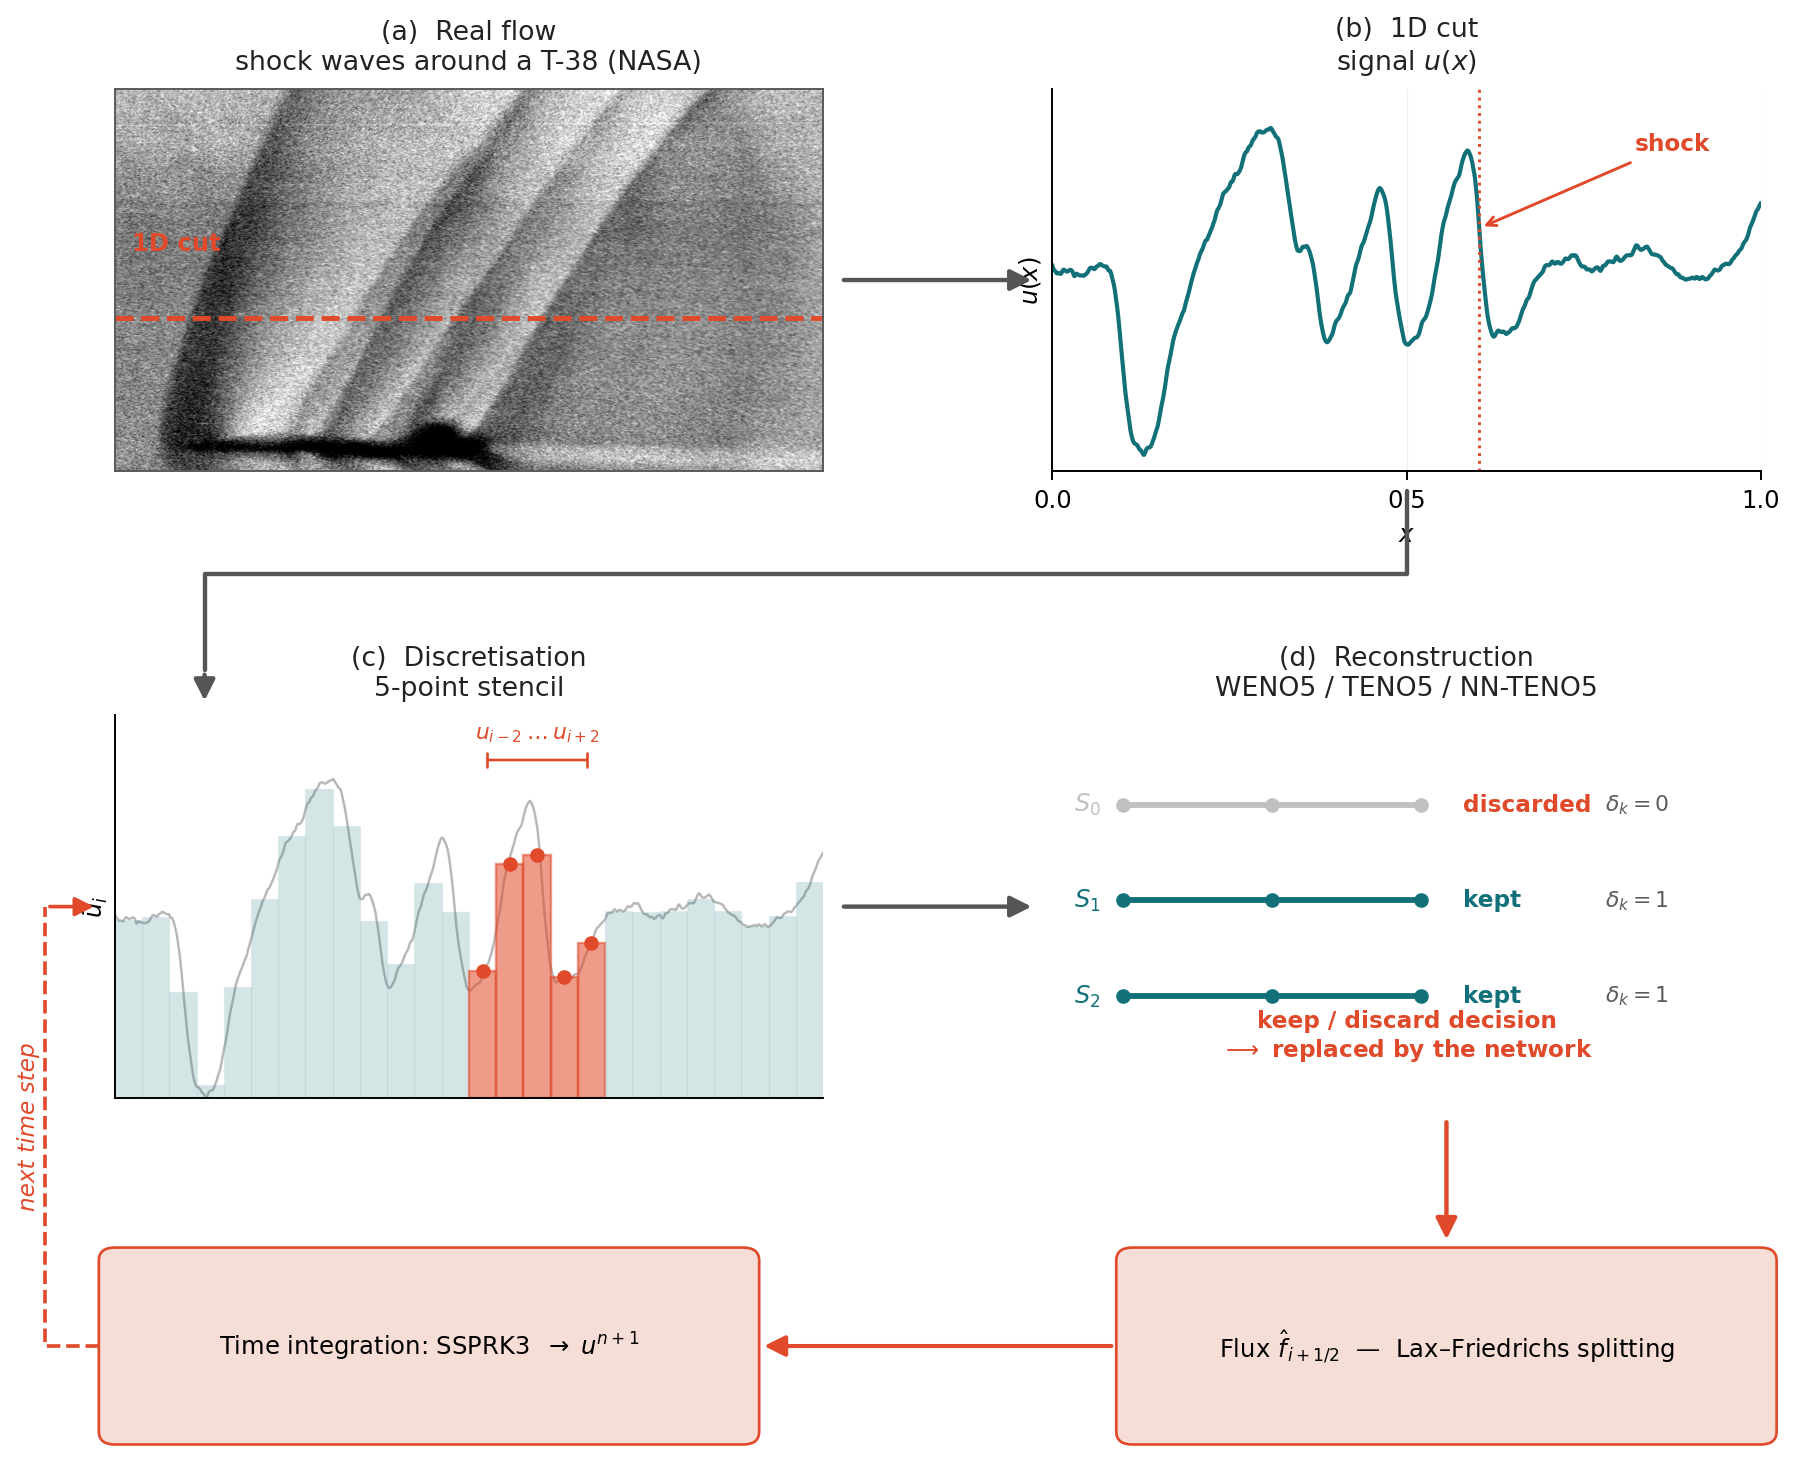
\includegraphics[width=\textwidth]{pipeline_visuel_en.png}
\caption{Complete computational chain, illustrated on a real case. (a) Shock
waves around a T-38 in supersonic flight (schlieren photograph,
NASA~\cite{nasa1993}) and the trace of a 1D cut. (b) The signal $u(x)$ actually
extracted from the pixels along that cut; the marker indicates the steepest
transition. (c) Discretisation into cells and the 5-point stencil centred on
that front. (d) The three TENO5 candidates: the one crossed by the
discontinuity is discarded ($\delta_k = 0$), the others are kept. The
reconstructed flux then feeds the Lax--Friedrichs splitting and the SSPRK3
integrator, and the loop resumes at the next step. \textbf{The internship bears
exclusively on the decision in panel~(d)}; every other link is identical
between the classical and the learned scheme.}
\label{fig:pipeline}
\end{figure}

The important point is that \textbf{the network intervenes at a single step
only}. It replaces neither the time integrator, nor the flux splitting, nor the
characteristic projection: it replaces solely the candidate-stencil selection
decision inside the reconstruction. This is what makes the comparison with the
classical scheme fair -- all other links are rigorously identical between the
two -- and it is also what imposes the project's central technical constraint:
to train the network against the result obtained \emph{after} several time
steps, the whole chain downstream of the reconstruction must be differentiable
(Section~\ref{sec:jax}).

\section{The benchmark problems}
\label{sec:problems}

Four canonical problems serve as the test bench throughout this report. They
are chosen because each isolates a different difficulty, and because they all
have an exact solution or a finely converged reference allowing an unambiguous
error measurement.

\subsection{Linear advection of a step}

The equation $\partial_t u + a\,\partial_x u = 0$ transports the initial
profile without deforming it: the exact solution at time $t$ is simply
$u_0(x - at)$. Any deformation observed is therefore \emph{entirely}
attributable to the numerical scheme, which makes it the cleanest possible
test. With a step as initial datum, the defect measured is \textbf{numerical
diffusion}: at each step the scheme slightly widens both fronts. Over a long
time this widening accumulates -- exactly what
Figure~\ref{fig:step-width} in Chapter~\ref{chap:work} shows.

\subsection{Burgers' equation}

The equation $\partial_t u + \partial_x (u^2/2) = 0$ adds
\textbf{nonlinearity}: the flux depends on the solution itself, so that
perfectly smooth initial data develops a shock in finite time. This problem
therefore tests the scheme's ability to handle a discontinuity it did not
receive as input but watched form on its own. In this report it plays an
additional role: since the flux function $u^2/2$ is absent from the original
training set, Burgers constitutes an explicit \textbf{out-of-distribution}
test.

\subsection{Sod's shock tube}

Sod's problem \cite{sod1978} is the reference test case for the Euler system.
Its initial datum is a simple discontinuity between two states at rest
(Figure~\ref{fig:sod-struct}a), as if a membrane separating a compressed gas
from an expanded one were ruptured at $t=0$.

\begin{figure}[H]
\centering
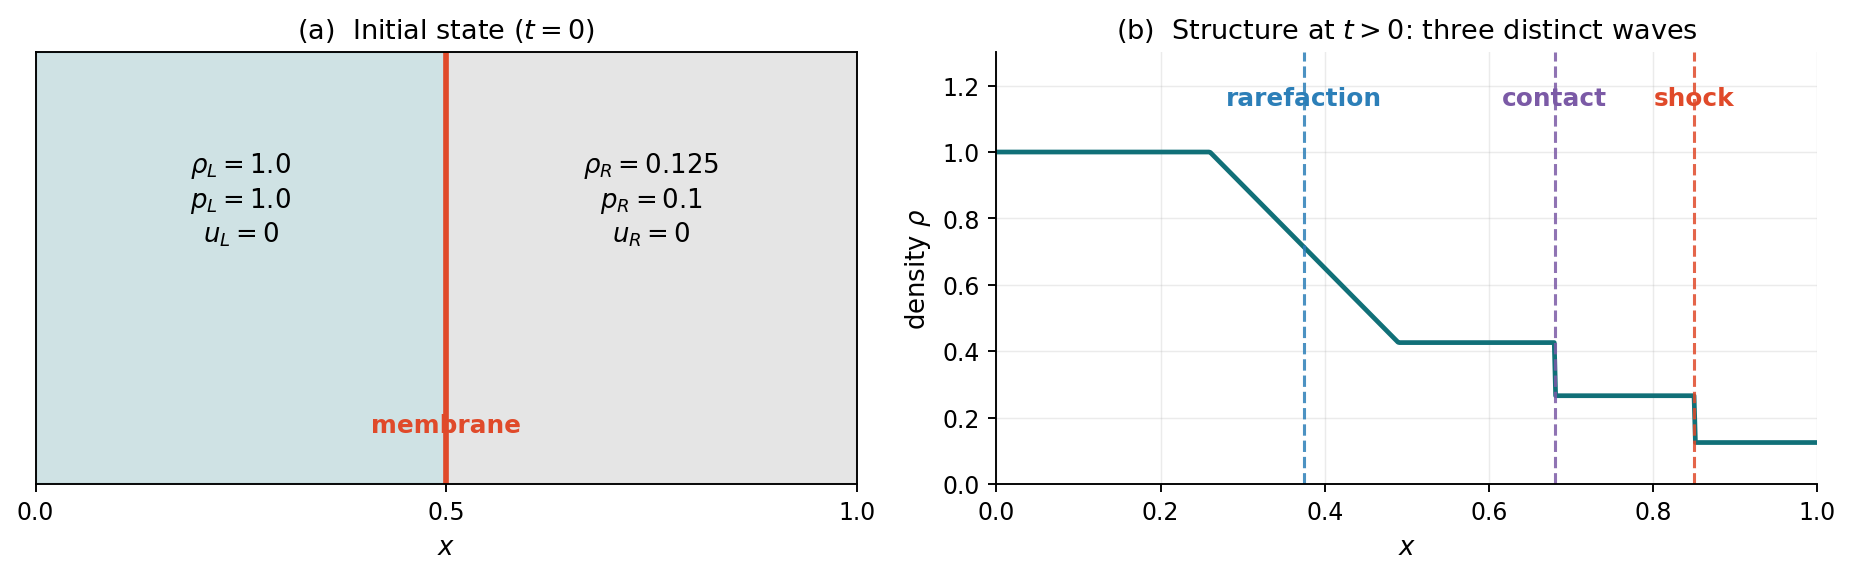
\includegraphics[width=\textwidth]{sod_structure_en.png}
\caption{Sod's shock tube. (a) Initial state: two states at rest separated by a
membrane. (b) Structure of the solution at $t>0$: the rupture simultaneously
generates three waves of different natures -- a smooth rarefaction, a contact
discontinuity and a shock.}
\label{fig:sod-struct}
\end{figure}

Its difficulty lies in the fact that the rupture generates \emph{three waves of
different natures simultaneously} (Figure~\ref{fig:sod-struct}b):

\begin{itemize}
  \item a \textbf{rarefaction wave}, smooth and spread out, which the scheme
  must resolve with its high order;
  \item a \textbf{contact discontinuity}, where density jumps but pressure and
  velocity remain continuous -- the hardest wave to keep sharp, since nothing
  in the dynamics opposes its diffusion;
  \item a \textbf{shock}, a sharp discontinuity, which the scheme must capture
  without oscillating.
\end{itemize}

A good scheme must therefore be simultaneously accurate, non-diffusive and
non-oscillatory, on three structures calling for opposite behaviours. It is
precisely because Sod is \emph{already very well handled} by TENO5 that it
proved, in this project, the problem most resistant to improvement by learning
(Section~\ref{sec:strand4}).

\subsection{The Shu--Osher problem}

The Shu--Osher problem is a shock propagating into a sinusoidal density field.
It thus combines, within a single computation, a \textbf{strong discontinuity}
and \textbf{fine oscillatory structures} -- a situation representative of
shock/turbulence interaction.

The difficulty does not come from the shock itself, which is captured without
trouble, but from the high-frequency oscillations located just behind it: an
overly dissipative scheme flattens them (see Figure~\ref{fig:shu-osher} in
Chapter~\ref{chap:work}). This is precisely the margin on which a learned
scheme can hope to gain, and it is indeed on this problem that the project's
only outright win on the Euler system was obtained.

This contrast between Sod and Shu--Osher -- one problem where the classical
scheme is already near-optimal, another where it leaves a dissipative margin --
is one of the report's structuring results, and is analysed in
Section~\ref{sec:strand4}.

\section{Related work}

Three published directions frame this work.

Stevens \& Colonius \cite{stevens2020} train a network to \emph{correct} the
WENO5 reconstruction rather than produce it from scratch: the network starts
from the classical scheme's result and learns only the deviation to apply to
it. Biasing the network this way, towards a known-good starting point, was
according to the authors the change that made training stable. This is a line
of reasoning the present project reuses directly, twice: for the imitation
pre-training (Section~\ref{sec:strand3}) and for the convex mixing mechanism
(Section~\ref{sec:strand4}).

Fu, Hu \& Adams \cite{fu2016} introduce the TENO scheme, whose selection
decision this internship seeks to improve.

Li, Fu \& Adams \cite{li2022} propose NENO6, which trains a
\emph{classifier} network predicting a troubled/keep probability per candidate.
Its architecture is the one adopted by this internship's NN-TENO5 classifier.

\section{Scope, assignment and methodology}

The topic, as stated on the internship specification sheet, was \emph{``Machine
learning-based numerical scheme for CFD''}, with three assignments: a
literature review, the construction of a neural network computing the weighting
functions of a WENO-type scheme, and the evaluation of its performance.

The scope was deliberately restricted to \textbf{one-dimensional} problems
(linear advection, Burgers' equation, the Euler system) and to fifth-order
schemes (WENO5, TENO5). Multi-dimensional extensions and higher orders
(WENO3/WENO7, TENO3/TENO7) were set aside for lack of time, and are discussed
as future work.

The work builds on an existing open-source codebase implementing the WENO5-NN
paper. Rather than starting from scratch, it extends that code to TENO5, first
reproduces its published results as a baseline, then tests a training
methodology absent from the published literature.

\subsection*{Working methodology}

Since the topic was a research question rather than a fixed specification, the
work was organised as a \textbf{sequence of falsifiable experiments} rather
than as a linear implementation plan: each phase proposes a precise mechanism,
tests it against the true solution, and keeps, fixes or abandons it according
to the measured result.

Two evaluation criteria were applied uniformly across all experiments:

\begin{itemize}
  \item \texttt{beats\_teacher}: the network's error against the true solution
  is strictly lower than the classical scheme's error against that same
  solution. \textbf{This is the only criterion used to claim a win in this
  report.}
  \item \texttt{teacher\_fidelity}: the network's error is within $2\%$ of the
  classical scheme's. This looser criterion was used only for early acceptance
  tests and is never used as evidence of superiority.
\end{itemize}

Every experiment was measured on canonical benchmarks (outside the training
data) and documented immediately, including when it made results worse. This is
why the project's internal experiment log records 21~phases rather than a
handful of selected successes: several fixes that were correct on paper turned
out to be measurably harmful and had to be reverted. A second methodological
rule, adopted after losing a working checkpoint, was to commit and back up
every verified good result before starting the next experiment.

Table~\ref{tab:tools} summarises the technical environment used.

\begin{table}[H]
\centering
\begin{tabularx}{\textwidth}{@{}lX@{}}
\toprule
\textbf{Category} & \textbf{Tools} \\
\midrule
Language & Python 3 \\
\rowrule
Numerical computing & NumPy, SciPy \\
\rowrule
Machine learning (phase 1) & TensorFlow / Keras \\
\rowrule
Differentiable learning (phase 2) & JAX, Optax \\
\rowrule
Visualisation & Matplotlib \\
\rowrule
Version control & Git \\
\rowrule
Writing & \LaTeX{} (XeLaTeX) \\
\bottomrule
\end{tabularx}
\caption{Technical environment of the project.}
\label{tab:tools}
\end{table}

% ============================================================
\chapter{Design of the Solution}
\label{chap:design}

\section{Overall code architecture}

The project is organised into modules that strictly separate the numerical
schemes, the networks and the differentiable layer:

\begin{itemize}
  \item \texttt{src/schemes/} -- deterministic NumPy implementations of WENO5
  and TENO5, serving both as reference schemes and as teachers for imitation
  training.
  \item \texttt{src/networks/} -- network definitions (Keras) and imitation
  training functions.
  \item \texttt{src/core/} -- solver: time integration, flux splitting,
  boundary conditions.
  \item \texttt{src/differentiable/} -- complete differentiable JAX rewrite of
  the numerical core (Section~\ref{sec:jax}).
  \item \texttt{scripts/} -- training, evaluation and figure-generation
  scripts.
\end{itemize}

\section{Architecture of the classifier network}
\label{sec:archi-network}

The NN-TENO5 network is a multilayer perceptron with five weight layers,
following the NENO6 architecture \cite{li2022}: a normalised 5-value stencil as
input, four ReLU hidden layers of decreasing width (64, 32, 16, 8), and a
sigmoid layer producing one troubled-probability per TENO5 candidate.
Figure~\ref{fig:archi} gives its detailed structure.

\begin{figure}[H]
\centering
\resizebox{\textwidth}{!}{%
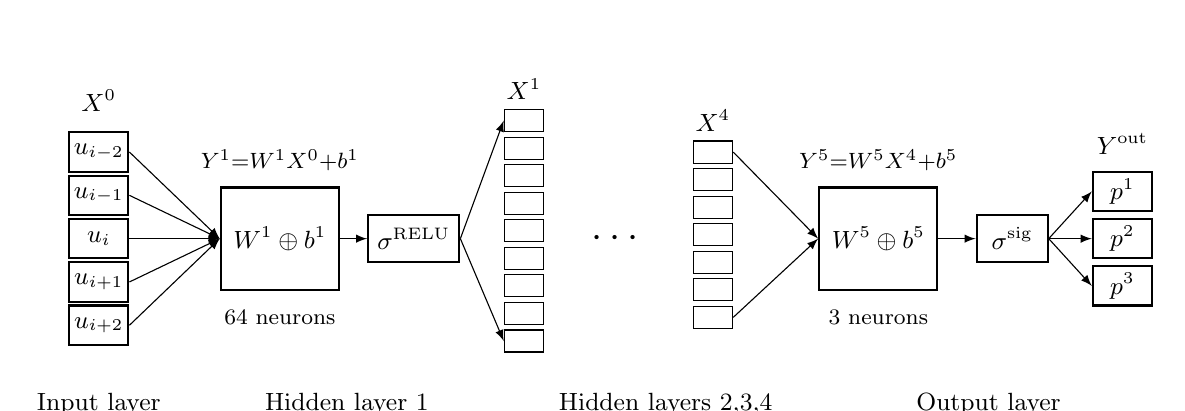
\begin{tikzpicture}[
  every node/.style={font=\small},
  iobox/.style={draw, thick, minimum width=0.75cm, minimum height=0.5cm, inner sep=1pt},
  bigbox/.style={draw, thick, minimum width=1.5cm, minimum height=1.3cm},
  smallbox/.style={draw, thick, minimum width=0.9cm, minimum height=0.6cm},
  stripe/.style={draw, thin, minimum width=0.5cm, minimum height=0.28cm, inner sep=0pt},
]
\foreach \i/\lab/\y in {1/u_{i-2}/1.1, 2/u_{i-1}/0.55, 3/u_i/0, 4/u_{i+1}/-0.55, 5/u_{i+2}/-1.1}{
  \node[iobox] (in\i) at (0,\y) {$\lab$};
}
\node at (0,1.75) {$X^0$};
\node[bigbox] (h1) at (2.3,0) {$W^1 \oplus b^1$};
\node at (2.3,-1.0) {\footnotesize 64 neurons};
\node at (2.3,1.0) {\footnotesize $Y^1{=}W^1X^0{+}b^1$};
\foreach \i in {1,...,5}{ \draw[-latex] (in\i.east) -- (h1.west); }
\node[smallbox] (relu1) at (4.0,0) {$\sigma^{\text{RELU}}$};
\draw[-latex] (h1.east) -- (relu1.west);
\foreach \k/\y in {1/1.5,2/1.15,3/0.8,4/0.45,5/0.1,6/-0.25,7/-0.6,8/-0.95,9/-1.3}{
  \node[stripe] (x1-\k) at (5.4,\y) {};
}
\node at (5.4,1.9) {$X^1$};
\draw[-latex] (relu1.east) -- (x1-1.west);
\draw[-latex] (relu1.east) -- (x1-9.west);
\node at (6.6,0) {\Large $\cdots$};
\foreach \k/\y in {1/1.1,2/0.75,3/0.4,4/0.05,5/-0.3,6/-0.65,7/-1.0}{
  \node[stripe] (x4-\k) at (7.8,\y) {};
}
\node at (7.8,1.5) {$X^4$};
\node[bigbox] (h5) at (9.9,0) {$W^5 \oplus b^5$};
\node at (9.9,-1.0) {\footnotesize 3 neurons};
\node at (9.9,1.0) {\footnotesize $Y^5{=}W^5X^4{+}b^5$};
\draw[-latex] (x4-1.east) -- (h5.west);
\draw[-latex] (x4-7.east) -- (h5.west);
\node[smallbox] (sig) at (11.6,0) {$\sigma^{\text{sig}}$};
\draw[-latex] (h5.east) -- (sig.west);
\foreach \i/\lab/\y in {1/p^1/0.6,2/p^2/0,3/p^3/-0.6}{
  \node[iobox] (out\i) at (13.0,\y) {$\lab$};
  \draw[-latex] (sig.east) -- (out\i.west);
}
\node at (13.0,1.2) {$Y^{\text{out}}$};
\node at (0,-2.1) {Input layer};
\node at (3.15,-2.1) {Hidden layer 1};
\node at (7.2,-2.1) {Hidden layers 2,3,4};
\node at (11.3,-2.1) {Output layer};
\end{tikzpicture}}
\caption{NN-TENO5 classifier architecture: a normalised 5-value stencil $X^0$
feeds four ReLU hidden layers of decreasing width (64, 32, 16, 8 neurons) then
a sigmoid layer, producing one troubled-probability $p^k$ per TENO5 candidate.}
\label{fig:archi}
\end{figure}

Each layer $l$ computes the same affine map $X^{l-1} \to Y^l = W^l X^{l-1} +
b^l$, followed by an activation:
\[
\sigma^{\text{RELU}}(x) = \max(x, 0), \qquad
\sigma^{\text{sig}}(x) = \frac{1}{1+e^{-x}}.
\]
The output $[p^1,p^2,p^3]$ reads as the probability that each candidate is
crossed by a discontinuity. At inference, a candidate is discarded as soon as
its probability exceeds $0.5$; during unrolled-loss training this hard
threshold is replaced by the continuous probability itself, so that gradients
can flow through the decision.

\section{The unrolled physics loss}
\label{sec:loss}

Imitation training has a structural limitation: its loss function only ever
measures the distance to the \emph{teacher's} decision, never the distance to
the \emph{true} solution. A network cannot be pushed towards an answer it is
never shown.

The supervisor proposed an alternative, the \textbf{unrolled physics loss}:
instead of a one-shot imitation label, the network is used to actually advance
the simulation over $K$ time steps, and the loss is computed directly against
the true solution $K$ steps later. It combines several terms, of which the
three main ones are:
\[
\mathcal{L}_{\text{total}} = \lambda_1\mathcal{L}_{\text{MSE}}
+ \lambda_2\mathcal{L}_{\text{TV}}
+ \lambda_3\mathcal{L}_{\text{Reg}} + \dots
\]
\[
\mathcal{L}_{\text{MSE}} = \frac{1}{N}\sum_{i=1}^{N}\left(u_i^{n+K} - u_{i,\text{exact}}^{n+K}\right)^2,
\qquad
\mathcal{L}_{\text{TV}} = \max\left(0,\ \mathrm{TV}(u^{n+K}) - \mathrm{TV}(u^{n})\right).
\]
The first, $\mathcal{L}_{\text{MSE}}$, measures the deviation from the true
solution after $K$ steps -- this is the central term, the one that makes the
approach different from imitation. The second penalises any increase in the
total variation $\mathrm{TV}(v) = \sum_i |v_{i+1}-v_i|$, that is, any
appearance of spurious oscillations. The third, $\mathcal{L}_{\text{Reg}}$,
anchors the network's solution to the classical scheme's and prevents it from
drifting arbitrarily away. To these is added a consistency term between
neighbouring cells (the \emph{Boundary Variation Diminishing} principle, or
BVD~\cite{fu2016}): at a given interface, the left cell and the right cell each
propose a value, and this term penalises their disagreement. Finally, for the
Euler system, a last term penalises non-physical states -- negative density or
pressure (Section~\ref{sec:instability}).

\section{The differentiable JAX rewrite}
\label{sec:jax}

This formulation could not be tested in the original code: unrolling $K$
simulation steps requires that the \emph{entire} chain -- reconstruction, flux
splitting, time integration, characteristic projection -- be differentiable end
to end. Yet the NumPy solver carries no gradient, and Keras'
\texttt{model.predict()} detaches entirely from the graph.

The \texttt{src/differentiable/} module is therefore a complete JAX rewrite of
the numerical core, not a mere wrapper. Table~\ref{tab:jax} summarises the
reimplemented components.

\begin{table}[H]
\centering
\begin{tabularx}{\textwidth}{@{}lX@{}}
\toprule
\textbf{Component} & \textbf{Content reimplemented in JAX} \\
\midrule
Reconstruction & complete TENO5: smoothness indicators, thresholding, renormalisation \\
\rowrule
Solver & SSPRK3, Lax--Friedrichs splitting, boundary conditions \\
\rowrule
Euler & characteristic projection, positivity repair \\
\rowrule
Network & forward pass of the MLP, with no dependency on Keras \\
\rowrule
Loss & all terms, including the Euler positivity penalty \\
\bottomrule
\end{tabularx}
\caption{Components rewritten in the differentiable JAX module.}
\label{tab:jax}
\end{table}

TENO5's binary thresholding poses a specific difficulty here: the function
$\delta_k$ has zero derivative almost everywhere, which would block any
backpropagation. This is why the network's continuous probability replaces the
hard threshold during training.

% ============================================================
\chapter{Implementation and Experiments}
\label{chap:work}

\section{Strand 1: WENO5-NN vs.\ WENO5}
\label{sec:strand1}

The first strand reproduces the three configurations published by Stevens \&
Colonius \cite{stevens2020}, from their original training set (75\,241
samples), in order to establish a verified baseline.

\textbf{Step advection.} WENO5-NN reduces the $L_1$ error by $28.7\%$, $L_2$ by
$17.1\%$, $L_\infty$ by $5.2\%$ and the shock width by $21.4\%$ compared with
WENO5: the clearest of the three cases. Figure~\ref{fig:step-width} explains
this gain: the width of the discontinuity produced by WENO5 grows continuously
under numerical diffusion, whereas the network's stabilises.

\begin{figure}[H]
\centering
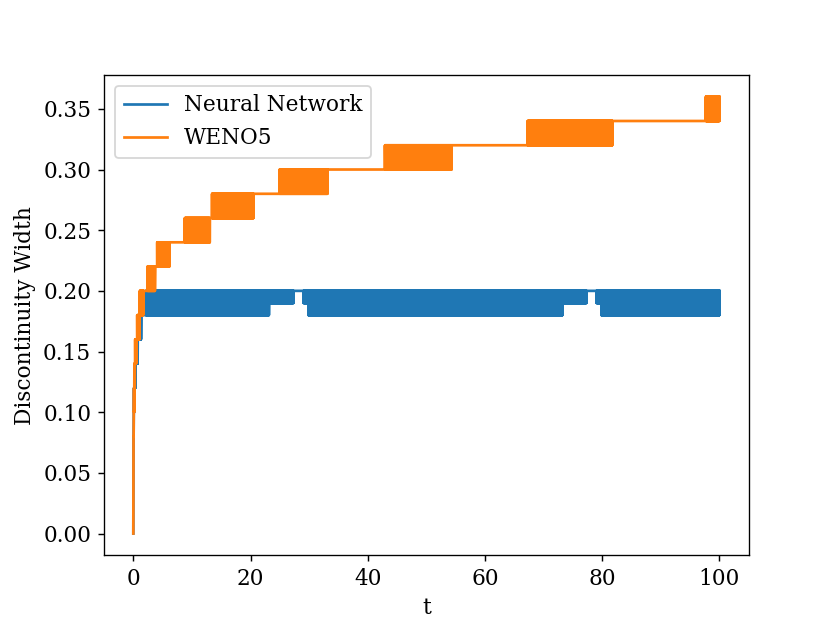
\includegraphics[width=0.60\textwidth]{step_advection/discontinuity_width_vs_time.png}
\caption{Discontinuity width as a function of time. WENO5's grows monotonically
under the effect of numerical diffusion; the network's stabilises around
$0.19$, which explains the $21.4\%$ gain measured at $t=100$.}
\label{fig:step-width}
\end{figure}

\textbf{Burgers' equation.} A distinctly mixed result: the network wins at
3~of the 4~resolutions tested and loses at the fourth
(Figure~\ref{fig:burgers-grid}). This matches the authors' own observation: the
two schemes behave similarly for a genuine shock, the network's advantage
coming mainly from the smooth pre-shock region.

\begin{figure}[H]
\centering
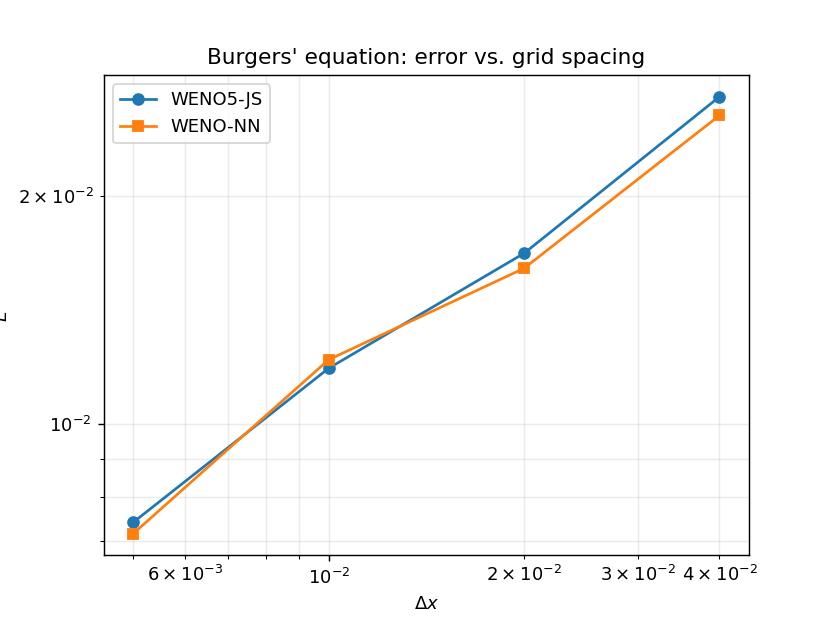
\includegraphics[width=0.56\textwidth]{burgers/error_vs_grid_spacing.png}
\caption{Burgers' equation: $L_2$ error as a function of grid spacing. The
network (orange) drops below WENO5-JS (blue) at three resolutions out of four,
and rises slightly above it around $\Delta x \approx 10^{-2}$.}
\label{fig:burgers-grid}
\end{figure}

\textbf{Sod and Shu--Osher.} Near-parity: the curves are visually
indistinguishable from the exact solution. It is nonetheless a loss under the
strict criterion, the network's $L_\infty$ error being higher by $0.265\%$ for
Sod and $0.551\%$ for Shu--Osher.

Strand~1's verdict is therefore a \textbf{strongly problem-dependent tie}: a
clear win where the network's training distribution matches the problem well,
and a near-parity loss on the cases that stress it more.

\section{Strand 2: NN-TENO5 by imitation vs.\ TENO5}
\label{sec:strand2}

The second strand applies the same idea to TENO5, with the classifier described
in Section~\ref{sec:archi-network}, trained to reproduce TENO5's keep/discard
decision.

By construction, a network trained solely to imitate a teacher cannot exceed
that teacher's reconstruction quality, except through its own generalisation
noise. The measurements confirm this: on 3~of the 4~scalar benchmarks tested,
NN-TENO5 produces an \emph{exact} tie with TENO5; on step advection it loses by
$0.64\%$; on the Euler benchmarks it produces two small wins compatible with
the imitation ceiling (reproducing or very slightly perturbing the teacher's
decision can occasionally land closer to the true solution by chance, without
systematic improvement).

Several attempts to break through within the imitation paradigm -- training on
an exact target, extending to a 7-point WENO7 stencil, an extensive
hyperparameter search, and training on ``oracle-relabelled'' TENO5 data -- all
produced either a negative result or a small win plateauing at the same level.
This finding, that \textbf{the ceiling is structural to the imitation paradigm
itself and not a tuning defect}, directly motivated the second phase of the
internship.

\section{Strand 3: scalar benchmarks with the unrolled loss}
\label{sec:strand3}

The unrolled loss was first tested on advection and Burgers. Three obstacles had
to be removed in sequence.

\textbf{Obstacle 1 -- imbalance between loss terms.} Training by following the
proposal's equations literally, with $\mathcal{L}_{\text{TV}}$ and
$\mathcal{L}_{\text{Reg}}$ unnormalised, lets the gradient of
$\mathcal{L}_{\text{TV}}$ dominate that of $\mathcal{L}_{\text{MSE}}$ by a
factor of about~4, even after applying its weight of $0.1$.
Figure~\ref{fig:loss-curves} shows the diagnosis and the effect of the fix
(normalising by the mean rather than the sum).

\begin{figure}[H]
\centering
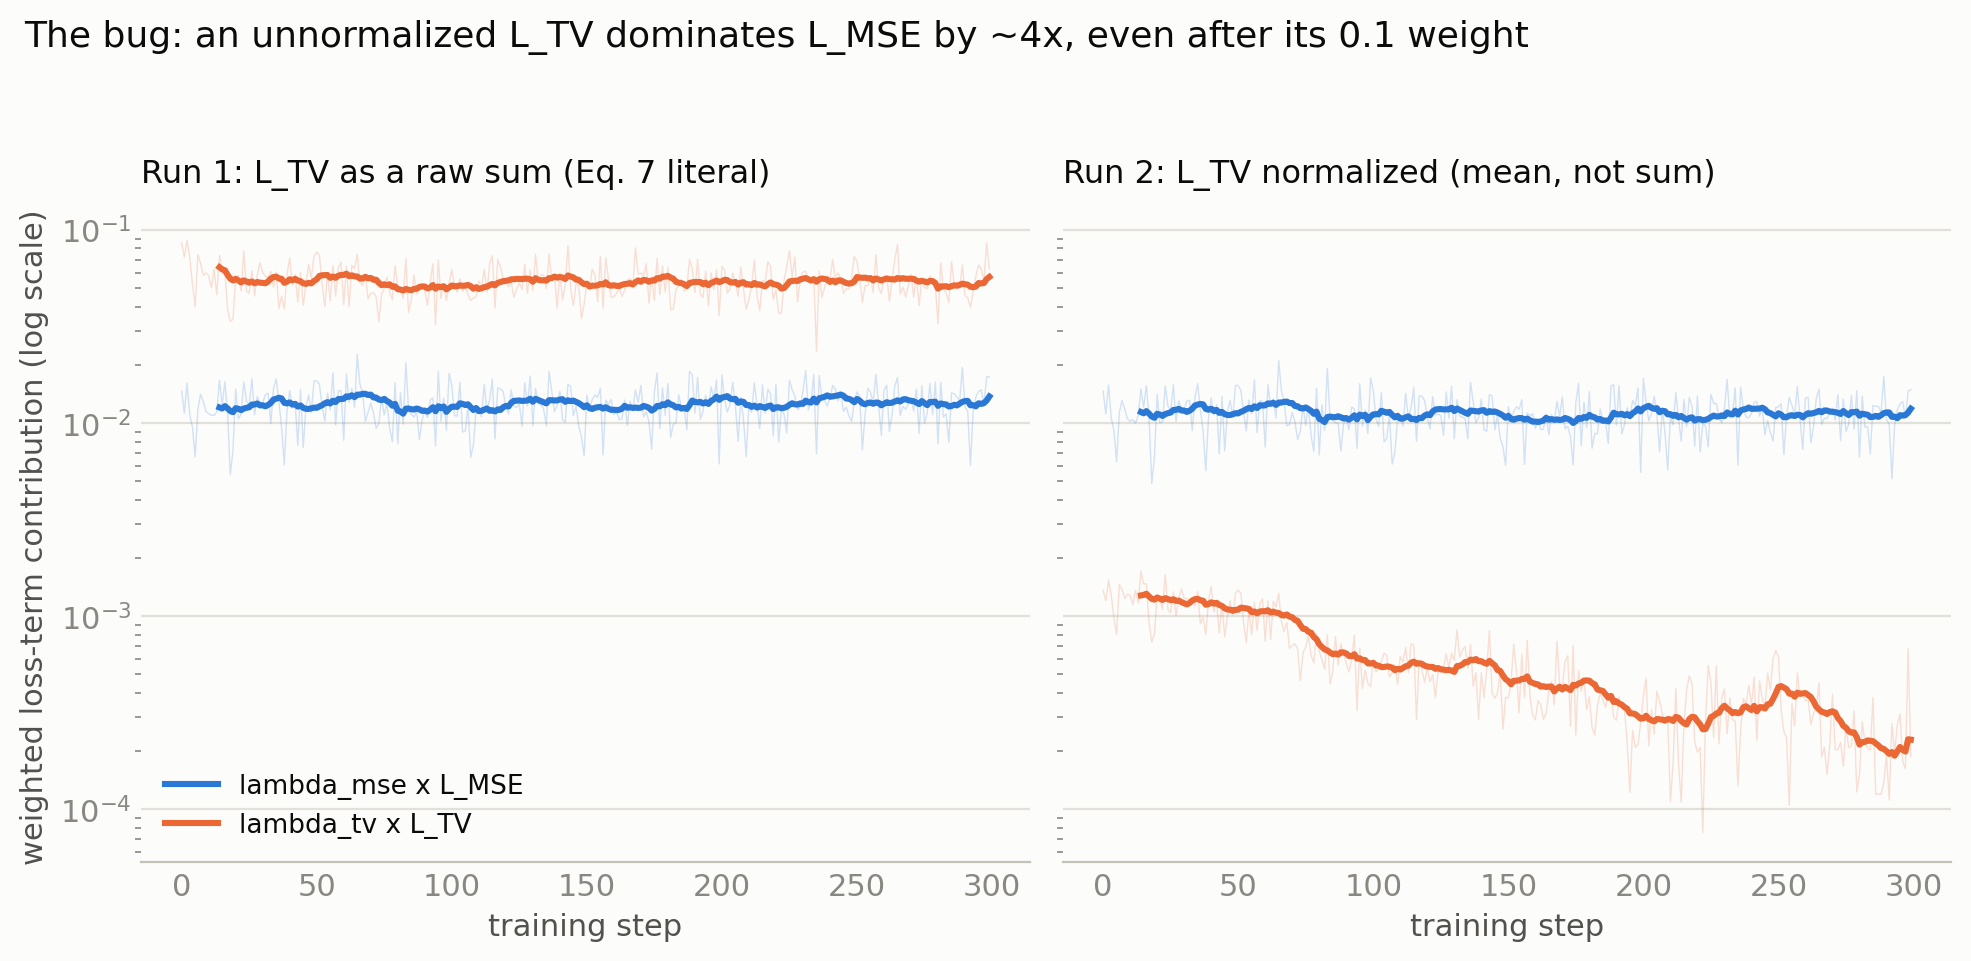
\includegraphics[width=\textwidth]{01_scalar_training_curves.png}
\caption{Weighted contributions of the loss terms during training. On the left,
the raw $\mathcal{L}_{\text{TV}}$ dominates $\mathcal{L}_{\text{MSE}}$ by about
a factor of~4 and training is in fact optimising the wrong quantity; on the
right, after normalisation, the expected balance is restored and
$\mathcal{L}_{\text{TV}}$ decreases.}
\label{fig:loss-curves}
\end{figure}

\textbf{Obstacle 2 -- initialisation.} Training a randomly initialised network
directly against the unrolled loss fails completely. The fix reuses the pattern
already validated in Strand~2: imitation pre-training, then fine-tuning with
the unrolled loss.

\textbf{Obstacle 3 -- generalisation.} The resulting network won 2~of the
3~held-out tests, but generalised neither to the full-scale canonical benchmark
nor to Burgers' nonlinear flux, absent from its training distribution.

The final fix reuses a mechanism developed first for the Euler system
(Section~\ref{sec:strand4}): a separately trained \textbf{mixing head}
producing a convex combination coefficient $\lambda \in [0,1]$ between TENO5's
reconstruction and the network's:
\[
u_{\text{final}} = (1-\lambda)\, u_{\text{TENO5}} + \lambda\, u_{\text{network}},
\]
complemented by Burgers-flux training examples. This mechanism guarantees that
the network can only interpolate \emph{towards} its own reconstruction from
TENO5's, never overshoot it in the wrong direction.

Two observations deserve emphasis. First, the \emph{untrained} head (with a
conservative initial bias giving $\lambda \approx 4.7\%$ uniformly) already won
on both canonical benchmarks \emph{before any additional training}. Second, and
counter-intuitively, \textbf{uniform mixing beats mixing concentrated on
troubled stencils}: letting the network also correct the classical scheme's
small errors in smooth regions yields more than confining it to the zones the
classical scheme flags.

\section{Strand 4: the Euler system}
\label{sec:strand4}

The Euler system is harder for two independent reasons: the reconstruction
there is coupled and characteristic-wise (Section~\ref{sec:background-fv}), and
the solution must remain physically valid (positive density and pressure) at
\emph{every} intermediate stage of training, not only at convergence.

\subsection{Diagnosis and correction of the instability}
\label{sec:instability}

The first training attempt diverged outright: state values grew without bound
within a few SSPRK3 substeps, however much the dissipation margin of the
Lax--Friedrichs splitting was increased. Figure~\ref{fig:instab} shows the
decisive result: \emph{increasing} dissipation makes the instability arrive
\emph{faster}, which rules out an under-resolved shock and points to a bug.

\begin{figure}[H]
\centering
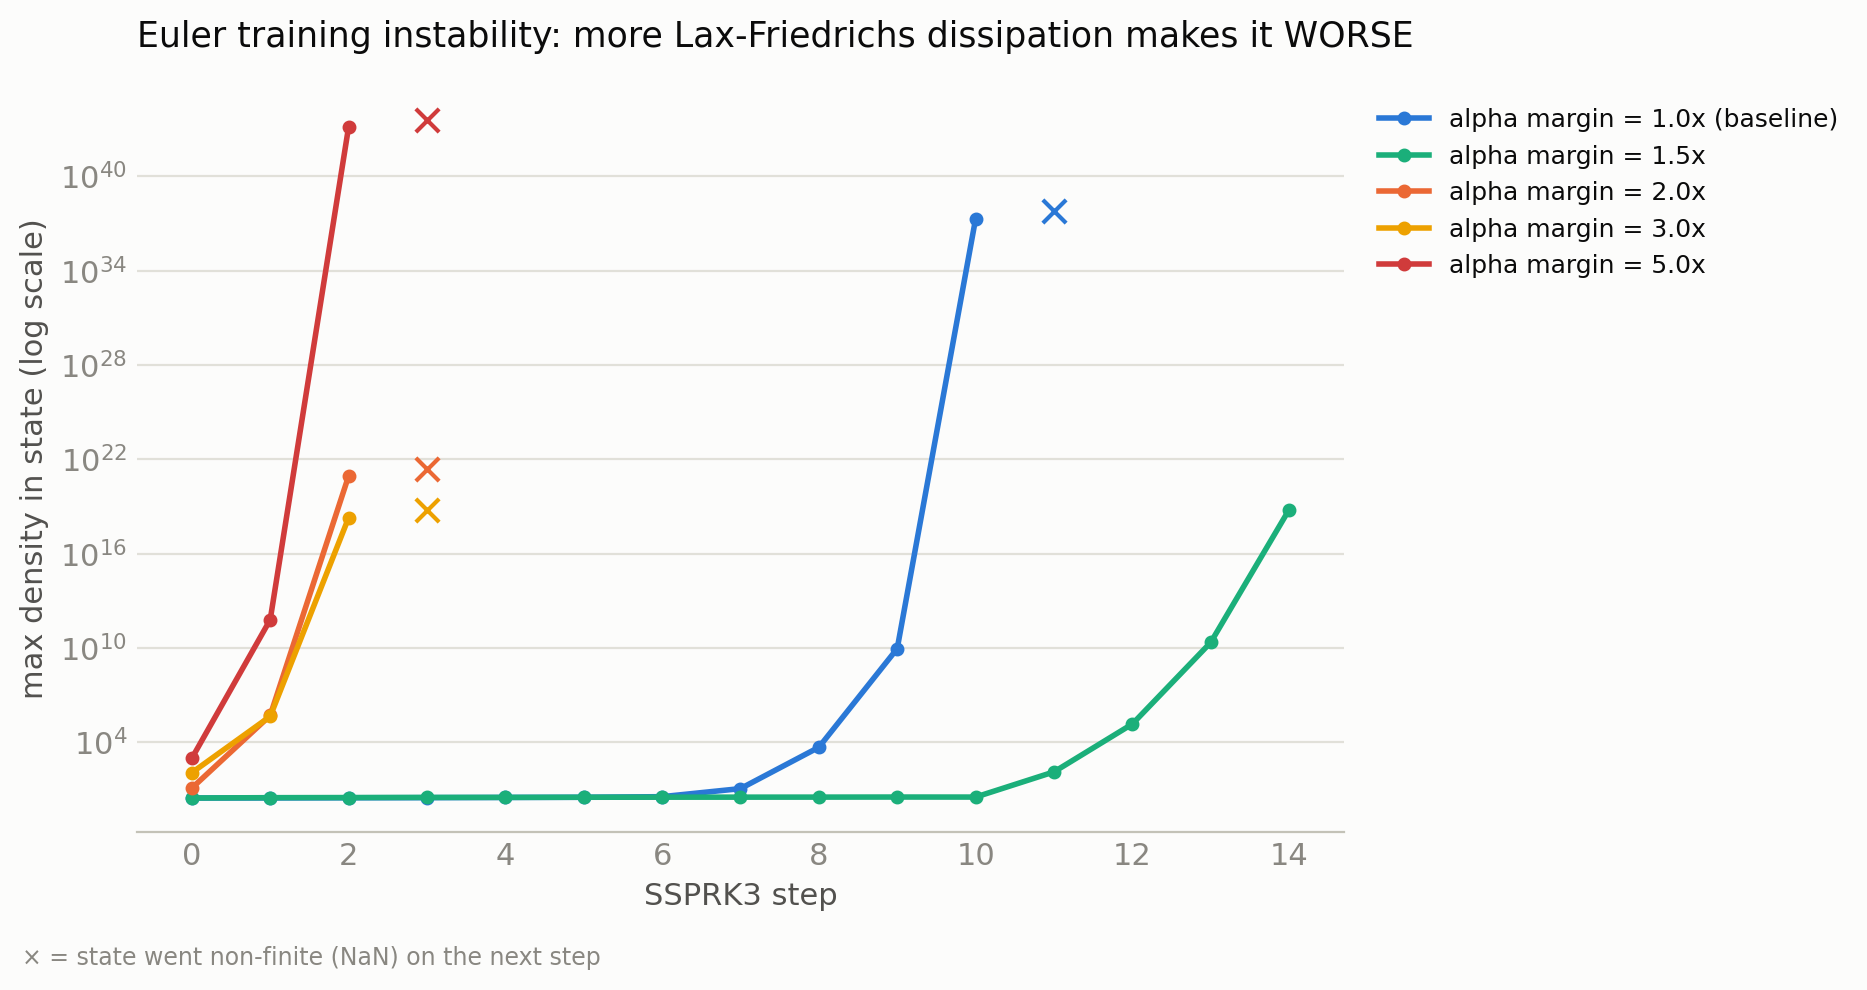
\includegraphics[width=0.72\textwidth]{04_euler_instability.png}
\caption{Training instability on Euler: the maximum density diverges all the
faster as the dissipation margin is increased. This counter-intuitive behaviour
rules out insufficient numerical dissipation as the cause and directs the
diagnosis towards the handling of positivity violations.}
\label{fig:instab}
\end{figure}

Two concrete defects were identified and fixed:

\begin{enumerate}
  \item \textbf{A structurally inert positivity penalty.} The term meant to
  penalise non-physical states was computed on the \emph{already-repaired}
  final state of each step, after a clamp had been applied: it could therefore
  mathematically never be nonzero. Fixed by computing the penalty on the
  substeps before repair.
  \item \textbf{An incomplete repair mechanism.} The repair checked only the
  sign; it detected neither non-finite values (\texttt{NaN}/\texttt{Inf}) nor
  unbounded magnitudes, which can arise from an imperfect reconstruction fed
  back into the next step's characteristic basis. Fixed by adding explicit
  finiteness and magnitude checks.
\end{enumerate}

Combined with the supervisor's clarification of the BVD term's definition,
these fixes produced the first Euler training run that does not diverge.

\subsection{The dedicated mixing head}

The mechanism that finally produced a canonical win is the convex mixing
introduced in Section~\ref{sec:strand3}, but its coefficient $\lambda$ had to
be computed by a \emph{dedicated} head, trained separately, rather than reused
from the network's troubled-probability output. Reusing that signal made
$\lambda$ carry two incompatible roles -- flagging trouble \emph{and}
calibrating the confidence placed in the network -- and caused three distinct
regressions. A small head trained specifically for this, initialised
conservatively (bias $=-3$, i.e.\ $\lambda \approx 4.7\%$ at the start), fixed
this and produced the project's first outright canonical win
(Figure~\ref{fig:shu-osher}).

\begin{figure}[H]
\centering
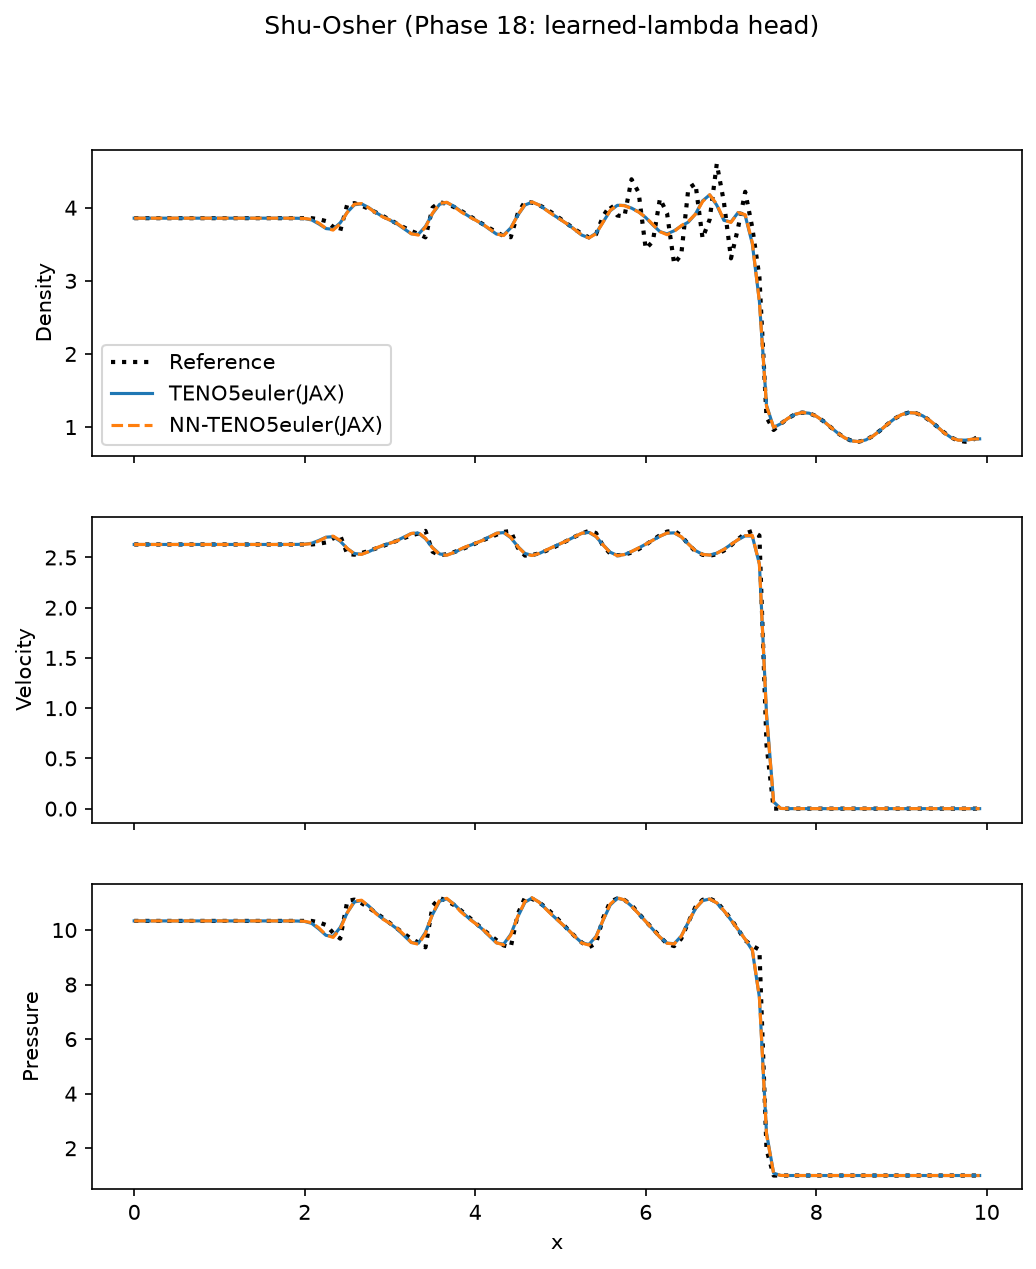
\includegraphics[width=0.56\textwidth]{euler_jax_comparison/shu_osher_phase18.png}
\caption{Shu--Osher with a dedicated mixing head: NN-TENO5euler and TENO5euler
are visually near-identical against the reference, with NN-TENO5euler being
$1.84\%$ more accurate in mean $L_1$ across the three conserved variables.}
\label{fig:shu-osher}
\end{figure}

The Sod case, by contrast, remained a near-tie slightly unfavourable to the
network even after this fix. Two further attempts -- a 50-fold higher learning
rate for the mixing head alone, and a richer gate seeing the raw stencil rather
than only the probability summary -- moved Sod's ratio only marginally
($1.0045\times$, then $1.0026\times$), never past parity.

A direct sweep of a fixed (non-learned) coefficient $\lambda$ confirmed that
this is a \textbf{structural limit} of the learned scheme on Sod, and not a
calibration defect: Sod's error increases \emph{monotonically} with every
$\lambda$ tested from $0$ to $0.3$, whereas Shu--Osher's \emph{decreases}
monotonically up to $\lambda \approx 0.2$ over the same sweep. No amount of
gate tuning can fix a backbone scheme that is, on this particular problem,
simply less accurate than TENO5.

% ============================================================
\chapter{Results, Critical Analysis and Limitations}
\label{chap:results}

\section{Evaluation metrics}
\label{sec:metrics}

All results are measured with the same set of metrics, applied identically to
the classical scheme and to the network. With $d_i = u_i - u_i^{\text{ref}}$:
\[
L_1 = \frac{1}{N}\sum_i |d_i|, \qquad
L_2 = \sqrt{\frac{1}{N}\sum_i d_i^2}, \qquad
L_\infty = \max_i |d_i|.
\]
For Euler, they are computed independently per conserved variable (density,
momentum, energy) and then averaged into a single scalar $\bar L_1$. Three
complementary diagnostics are used: the total variation
$\mathrm{TV}(u)=\sum_i|u_{i+1}-u_i|$ (an excess of which signals a spurious
oscillation), positivity ($\min_i \rho_i > 0$ and $\min_i p_i > 0$), and the
localisation error of the shock and of the contact.

\section{Consolidated results}
\label{sec:consolidated}

Tables~\ref{tab:strand3} and~\ref{tab:strand4} consolidate the final
measurements, and Table~\ref{tab:summary} summarises the four strands.

\begin{table}[H]
\centering
\begin{adjustbox}{max width=\textwidth}
\begin{tabular}{lrrrl}
\toprule
\textbf{Benchmark} & \textbf{TENO5} & \textbf{NN-TENO5 (JAX)} & \textbf{Ratio} & \textbf{Verdict} \\
\midrule
Advection ($L_1$) & 3.4819e-02 & 3.3813e-02 & $0.9711\times$ & \textbf{WIN} \\
\rowrule
Advection ($L_2$) & 9.8960e-02 & 9.5521e-02 & $0.9653\times$ & \textbf{WIN} \\
\rowrule
Burgers ($L_1$, out of distribution) & 2.0697e-04 & 1.7873e-04 & $0.8636\times$ & \textbf{WIN} \\
\rowrule
Burgers ($L_2$, out of distribution) & 8.1670e-04 & 6.6493e-04 & $0.8142\times$ & \textbf{WIN} \\
\bottomrule
\end{tabular}
\end{adjustbox}
\caption{Strand~3 (scalar), canonical-scale evaluation. NN-TENO5 wins on both
benchmarks, including Burgers, explicitly outside the training distribution.}
\label{tab:strand3}
\end{table}

\begin{table}[H]
\centering
\begin{adjustbox}{max width=\textwidth}
\begin{tabular}{lrrrl}
\toprule
\textbf{Benchmark} & \textbf{TENO5euler $\bar L_1$} & \textbf{NN-TENO5euler $\bar L_1$} & \textbf{Ratio} & \textbf{Verdict} \\
\midrule
Sod & 8.2583e-03 & 8.2871e-03 & $1.0035\times$ & LOSS \\
\rowrule
Shu--Osher & 2.1319e-01 & 2.0926e-01 & $0.9816\times$ & \textbf{WIN} \\
\bottomrule
\end{tabular}
\end{adjustbox}
\caption{Strand~4 (Euler), best model obtained (dedicated mixing head). Sod is
$0.35\%$ less accurate; Shu--Osher is $1.84\%$ more accurate -- the first
outright win against a classical scheme on a canonical benchmark obtained in
this project.}
\label{tab:strand4}
\end{table}

\begin{table}[H]
\centering
\small
\begin{tabularx}{\textwidth}{@{}>{\raggedright\arraybackslash}p{0.20\textwidth}>{\raggedright\arraybackslash}p{0.20\textwidth}>{\centering\arraybackslash}p{0.10\textwidth}>{\raggedright\arraybackslash}X@{}}
\toprule
\textbf{Strand} & \textbf{Verdict} & \textbf{Result} & \textbf{Main observation} \\
\midrule
1. WENO5-NN vs.\ WENO5 & Strongly problem-dependent & TIE & Win on advection and 3/4 Burgers resolutions; slight loss on Sod and Shu--Osher. \\
\rowrule
2. NN-TENO5 (imitation) & Reproduces its teacher & TIE & Three exact ties, two small Euler wins, one loss on advection. \\
\rowrule
3. NN-TENO5 (unrolled loss), scalar & Win on both benchmarks & \textbf{WIN} & $3.5\%$ on advection, $18.6\%$ on Burgers (out of distribution). \\
\rowrule
4. NN-TENO5euler (unrolled loss) & First canonical win & \textbf{WIN} & $1.84\%$ on Shu--Osher; Sod remains a structural near-tie. \\
\bottomrule
\end{tabularx}
\caption{Overall summary of the four strands.}
\label{tab:summary}
\end{table}

\section{Critical analysis}

Two results stand out, and they are two faces of the same observation:
\textbf{how a network is trained matters more than its architecture}.

The first is Strand~2's imitation ceiling. A network trained to copy a teacher
inherits its limits; no amount of hyperparameter tuning, stencil widening or
relabelling made it possible to break through. The second is the success of
Strands~3 and~4: by changing the training \emph{signal} -- a loss measured
against the true solution after $K$ real steps, rather than against a teacher's
decision -- the same type of network becomes able to surpass the classical
scheme, including on a flux absent from its training distribution.

Three reservations must nonetheless accompany these results.

\textbf{The gains are modest and not uniform.} $1.84\%$ on Shu--Osher is a real
but small win, and Sod remains unfavourable. The $\lambda$ sweep shows that the
behaviour is of opposite sign on the two problems, suggesting that the learned
scheme does not improve the reconstruction universally, but only on certain
flow structures.

\textbf{The computational cost is not offset.} Every neural variant runs
markedly slower per cell than its classical equivalent -- roughly $5$ to
$18\times$ for the Keras-based models. The accuracy gains reported are
therefore not, as things stand, a cost/accuracy advantage.

\textbf{The winning mechanism is a safeguard.} The convex mixing head
guarantees that the network can only interpolate towards its own reconstruction
without overshooting it. This is what makes the result robust, but it also
mechanically bounds the attainable improvement.

\section{Limitations and future work}

The work remained limited to one-dimensional problems, scalar and Euler, and to
fifth-order schemes. Three natural extensions emerge:

\begin{itemize}
  \item \textbf{Extension to WENO7/TENO7 and to 2D.} The differentiable stack
  and the convex mixing mechanism are independent of order and dimension; their
  extension is essentially an engineering task.
  \item \textbf{Reducing inference cost.} The current overhead comes from an
  unoptimised implementation; distillation into a smaller network, or dedicated
  compilation, are direct avenues.
  \item \textbf{Understanding the Sod / Shu--Osher asymmetry.} Identifying
  which flow characteristic makes mixing beneficial in one case and harmful in
  the other would be the scientifically most useful extension, and might allow
  $\lambda$ to be conditioned on that characteristic.
\end{itemize}

% ============================================================
\chapter*{Conclusion}
\addcontentsline{toc}{chapter}{Conclusion}
\markboth{Conclusion}{}

The aim of this internship was to determine whether a neural network can
improve a classical shock-capturing numerical scheme, measured strictly against
the true solution. The answer obtained is nuanced but positive, and it depends
above all on \emph{how} the network is trained.

The first two strands, based on imitation training, end in a tie: reproducing
the published WENO5-NN results confirms their strongly problem-dependent
character, and extending the approach to TENO5 reveals a structural ceiling --
a network that copies a teacher cannot surpass it. This negative result was the
turning point of the internship.

The following two strands, based on the unrolled physics loss proposed by the
supervisor, break through that ceiling. They required a complete,
differentiable rewrite of the numerical core in JAX, without which the proposal
was not testable. They lead to verified wins on the canonical scalar benchmarks
($3.5\%$ on advection, $18.6\%$ on Burgers, out of distribution) and to a first
outright win on the Euler system ($1.84\%$ on Shu--Osher), obtained through a
dedicated convex mixing head. The Sod case remains unfavourable, and a direct
sweep of the mixing coefficient establishes that this is a structural limit of
the learned scheme.

On a personal level, this internship was formative above all through its
experimental discipline. The most useful results were not the wins but the
diagnoses: understanding why increasing dissipation worsened the instability
led to a structurally inert loss term; understanding why the network plateaued
led to the change of training paradigm. I also learned to treat a negative
result as data to be documented rather than a failure to be hidden -- that is
what made progress measurable, and it is the skill I take away most clearly
from these two months.

% ============================================================
\begin{thebibliography}{9}
\addcontentsline{toc}{chapter}{References}

\bibitem{harten1987}
A.~Harten, B.~Engquist, S.~Osher, S.~R.~Chakravarthy.
\emph{Uniformly high order accurate essentially non-oscillatory schemes,~III}.
Journal of Computational Physics, 71(2):231--303, 1987.

\bibitem{shu1988}
C.-W.~Shu, S.~Osher.
\emph{Efficient implementation of essentially non-oscillatory shock-capturing
schemes}.
Journal of Computational Physics, 77(2):439--471, 1988.

\bibitem{jiang1996}
G.-S.~Jiang, C.-W.~Shu.
\emph{Efficient implementation of weighted ENO schemes}.
Journal of Computational Physics, 126(1):202--228, 1996.

\bibitem{borges2008}
R.~Borges, M.~Carmona, B.~Costa, W.~S.~Don.
\emph{An improved weighted essentially non-oscillatory scheme for hyperbolic
conservation laws}.
Journal of Computational Physics, 227(6):3191--3211, 2008.

\bibitem{fu2016}
L.~Fu, X.~Y.~Hu, N.~A.~Adams.
\emph{A family of high-order targeted ENO schemes for compressible-fluid
simulations}.
Journal of Computational Physics, 305:333--359, 2016.

\bibitem{stevens2020}
B.~Stevens, T.~Colonius.
\emph{Enhancement of shock-capturing methods via machine learning}.
Theoretical and Computational Fluid Dynamics, 34:483--496, 2020.

\bibitem{li2022}
Y.~Li, L.~Fu, N.~A.~Adams.
\emph{A six-point neuron-based ENO (NENO6) scheme for compressible fluid
dynamics}.
arXiv:2207.08500, 2022.

\bibitem{wen2020}
X.~Wen, W.~S.~Don, Z.~Gao, J.~S.~Hesthaven.
\emph{An edge detector based on artificial neural network with application to
hybrid Compact-WENO finite difference scheme}.
Journal of Scientific Computing, 83(49), 2020.

\bibitem{sod1978}
G.~A.~Sod.
\emph{A survey of several finite difference methods for systems of nonlinear
hyperbolic conservation laws}.
Journal of Computational Physics, 27(1):1--31, 1978.

\bibitem{jax2018}
J.~Bradbury, R.~Frostig, P.~Hawkins, et al.
\emph{JAX: composable transformations of Python+NumPy programs}.
\url{http://github.com/google/jax}, 2018.

\bibitem{nasa1993}
L.~Weinstein / NASA.
\emph{Schlieren photograph of T-38 shock waves} (Mach~1.1, 13\,000~ft).
NASA Dryden Flight Research Center Photo Collection, photo EC94-42528-1,
13~December 1993. Public domain (work of the U.S. Government).
Available on Wikimedia Commons:
\url{https://commons.wikimedia.org/wiki/File:Schlieren_photograph_of_T-38_shock_waves.jpg}

\end{thebibliography}

% ============================================================
% BACK COVER
% ============================================================
\cleardoublepage
\thispagestyle{empty}
\null\vfill
\begin{center}
{\color{umorange}\rule{0.8\textwidth}{1pt}}

\vspace{0.9cm}
{\Large\bfseries\color{accent} Machine-Learning-Augmented\\[4pt]
Shock-Capturing Schemes}

\vspace{0.5cm}
{\color{umorange}\rule{0.8\textwidth}{1pt}}
\vspace{1.2cm}

\begin{minipage}{0.82\textwidth}
\small
This report investigates whether a neural network can improve the
reconstruction step of a classical shock-capturing numerical scheme (WENO5,
TENO5) for hyperbolic conservation laws, evaluated strictly against the true
solution on canonical benchmarks.

\vspace{0.5em}
The work first establishes a structural ceiling: a network trained to imitate a
teacher scheme's decision cannot surpass it. It then breaks through that
ceiling by means of an unrolled physics loss, which evaluates the network after
$K$ real simulation steps against the true solution -- a formulation that
required a complete, differentiable rewrite of the solver in JAX. The result is
a verified win on the canonical scalar benchmarks and a first outright win on
the Euler system.
\end{minipage}

\vspace{1.6cm}

\textbf{Keywords:} WENO, TENO, shock capturing, conservation laws,\\
deep learning, automatic differentiation, JAX, Euler system.

\vspace{2.2cm}


\includegraphics[width=0.36\textwidth]{um6p_college_of_computing_logo.png}

\vspace{0.5cm}
{\small Mohammed~VI Polytechnic University -- College of Computing\\
Academic year 2025--2026}
\end{center}
\vfill

\end{document}
